\chapter{REVISÃO BIBLIOGRÁFICA}
\label{cap1Revisao}

Na América Latina, historicamente marcada por colônias de exploração, o extrativismo mineral teve início para atender aos interesses dos países colonizadores, continuando ao longo dos anos. No final da década de 1990, com a expansão da globalização e o aumento do consumo de metais, a indústria mineral começou a se expandir em ritmo acelerado, tanto em termos de volumes extraídos quanto na abertura de novas minas \cite{fernandes2016mineracao}.

Em 2023, o Brasil estava entre um dos principais produtores de minerais do mundo, ocupando a nona posição no ranking dos 20 principais países em termos de valor na produção de minerais metálicos e carvão \cite{wpr2024mineral}. Este setor possui significativa importância na economia nacional, gerando emprego e desempenhando um papel crucial nas exportações do país, com uma alta comercialização de commodities \cite{rbm2024mineracao}.

A atividade mineral apresenta potencial significativo para incrementar a arrecadação tributária e fomentar o crescimento econômico, além de proporcionar melhorias na qualidade de vida da população e promover o desenvolvimento regional, conforme argumentam \citeauthor{carvalho2012dependencia} (\citeyear{carvalho2012dependencia}, p. 1), o setor mineral possui relevância estratégica por sua presença em diversos segmentos econômicos, ``produzindo bens primários, que irão suprir as mais variadas atividades econômicas, desde a agricultura até indústrias de tecnologia de ponta''. Os autores ressaltam ainda, que
economias que possuem como base a extração dos recursos minerais têm a mineração como fator fundamental.

\section{Atividade de Mineração}
\label{sec:atividade_mineracao}

A história da mineração no Brasil está intrinsecamente ligada a outras regiões do mundo, contribuindo conjuntamente para o desenvolvimento do sistema econômico amplamente conhecido como capitalismo \cite[p. 5]{domingues2022historia}.

Durante séculos, a exploração de recursos minerais no continente latino-americano constituiu uma base fundamental da economia do Antigo Sistema Colonial, tanto para Portugal quanto para a Espanha. A região mineradora de Potosí, atual Bolívia, por exemplo, destacou-se como o principal centro de extração de prata na América Latina destinada à Europa durante os séculos XVI e XVII. Essa região ``forneceu metade de toda a prata que saiu da América com destino à Espanha ao longo do período colonial'' \cite[p. 122]{araoz2020mineracao}. No território controlado pelo Estado português, segundo \citeauthor{figueiroa1997ciencias} (\citeyear{figueiroa1997ciencias}, p. 38), cinquenta por cento da produção mundial de ouro nos séculos XV e XVIII proveio dessa área.

O início da exploração de minérios no continente latino-americano acompanhou as políticas de desenvolvimento das nações europeias, fornecendo os recursos necessários para a ocorrência da 'Revolução Industrial'. A própria história da escravidão moderna e dos povos indígenas está interligada a esse processo. Em Potosí, por exemplo, utilizava-se a exploração da mão de obra indígena por meio do sistema conhecido como 'mita'. Já nas minas da região de Minas Gerais, a exploração era realizada com trabalho escravo oriundo das sociedades africanas \cite[p. 5]{domingues2022historia}.

A mineração no Brasil deu início no século XVII, durante o período colonial, quase dois séculos após a chegada dos portugueses em território sul-americano. A demora na descoberta de jazidas minerais significativas sugere que os interesses econômicos portugueses estavam primariamente voltados para a exploração de recursos como madeira (especialmente pau-brasil), cultivos como o açúcar e o tabaco, bem como para o uso de mão de obra escrava. Estes recursos foram os principais impulsionadores da economia colonial brasileira até que a descoberta de jazidas minerais, como ouro e diamantes, nas regiões de Minas Gerais, Goiás e Mato Grosso, alterou significativamente o foco econômico da colônia, sendo o primeiro grande \textit{boom} mineral, levando o Brasil a se tornar o principal produtor mundial de ouro durante os séculos XVIII e XIX \cite[p. 5]{barreto2001mineracao}; com os resultados da exploração dessa região, a coroa portuguesa superou o volume explorado pela Espanha, marcando o período conhecido pela historiografia como o 'Ciclo do Ouro' \cite[p. 6]{domingues2022historia}.

A mineração em Minas Gerais, assim como em muitas outras regiões da América Latina, desempenhou um papel fundamental na organização e expansão do sistema financeiro e comercial do capitalismo na Europa. Dessa forma, os recursos minerais dessa parte do continente americano foram componentes essenciais para a ``expansão do socio metabolismo urbano-industrial europeu'' \cite[p. 181]{araoz2020mineracao}.

Após quase um século de exploração intensiva, o primeiro ciclo de ouro no Brasil começou a declinar devido ao esgotamento das jazidas superficiais. Segundo \citeauthor{figueiroa1997ciencias} (\citeyear{figueiroa1997ciencias}, p. 38), a extração do ouro de 1750 para 1785 foi de uma média de mais de quinze (15) toneladas por ano para menos de cinco (5) toneladas. Diante dessa realidade, os esforços foram redirecionados para criação de condições favoráveis para a instalação de grandes empresas estrangeiras, principalmente inglesas, no país. Assim, durante o século XIX, teve início, embora com pouco sucesso inicial, um novo ciclo de busca por jazidas primárias de ouro, marcando uma transição na indústria mineral brasileira e estabelecendo as bases para futuras explorações e desenvolvimento no setor.

A mineração desempenha um papel fundamental no desenvolvimento do sistema capitalista, sendo um eixo central na prosperidade da tecnologia industrial. No Brasil, esse desenvolvimento adquire contornos significativos, no século XX, ganhando ímpeto após o término da Segunda Guerra Mundial, durante o governo de Getúlio Vargas na década de 1930, caracterizado pela intervenção do Estado nos setores da economia. Segundo \citeauthor{barreto2001mineracao}, as descobertas mais marcantes do século XX foram:

\begin{quotation}
o manganês da Serra do Navio (anos 40); o petróleo, que culminou com a criação da Petrobras (anos 50); as jazidas ferríferas do vale do Paraopeba (anos 50); as minas do Quadrilátero Ferrífero de Minas Gerais (meados dos anos 50, intensificando-se nos anos 60); o carvão no Rio Grande do Sul e no Paraná (anos 50), com grande incremento a partir dos anos 60; as minas de cobre do Rio Grande do Sul (anos 60), Pará e Goiás, nas décadas posteriores; as minas de chumbo na Bahia (anos 60), e em Minas Gerais mais recentemente; o nióbio de Araxá em Minas Gerais (anos 60); o caulim na Amazônia; fosfato e zinco em Minas Gerais; o megaprojeto Carajás no Pará; o amianto da mina Cana Brava, em Goiás; a bauxita de Minas Gerais e Pará; assim como a descoberta da província estanífera de Rondônia, todos na década de 1970 \cite[p. 6]{barreto2001mineracao}.
\end{quotation}

Nesse contexto político e econômico, desenvolvem-se as indústrias de base no Brasil, responsáveis pela transformação de matéria-prima bruta, como a fundição de ferro, alumínio e cobre, além da extração e fabricação de cimento, entre outros processos industriais \cite[p. 7]{domingues2022historia}.

A partir dessas circunstâncias históricas na década de 1930, o Estado brasileiro criou códigos legislativos para intervir jurídica e economicamente nas relações entre a indústria, o Estado e o meio natural. Exemplos dessas intervenções incluem o Decreto Federal nº 24.642, de 10 de julho de 1934, que regulamenta o uso das jazidas na mineração, o Decreto Federal nº 24.643, de 10 de julho de 1934, que trata da utilização das águas e continua em vigor até os dias atuais, e o Código Florestal de 1934, estabelecido pelo Decreto Federal nº 23.793, de 23 de janeiro de 1934.

A demanda do Estado pela atividade mineradora, visando o desenvolvimento da industrialização no contexto mencionado, resultou na concessão de concessões legais à iniciativa privada para explorar as jazidas, além da criação de grandes empresas mineradoras estatais. Em 1941, foi criada a Companhia Siderúrgica Nacional (CSN), em Volta Redonda, que se destacou na exploração das jazidas de minério de ferro, entre outras atividades. Em 1942, o Estado estabeleceu outra grande mineradora, a Companhia Vale do Rio Doce (CVRD), ambas constituídas como empresas estatais, sendo fornecedoras de aço e desempenhando um papel fundamental no desenvolvimento da indústria brasileira \cite[p. 8]{domingues2022historia}.

No Brasil, o segundo ciclo significativo na exploração mineral do Brasil, notadamente a partir da década de 1950, e alcançando sua efetiva consolidação no final dos anos 1960. De acordo com \citeauthor{fonseca2012progresso} (\citeyear{fonseca2012progresso}, p. 51-56), esse período foi marcado pela defesa da industrialização, pelo intervencionismo pró-crescimento e pelo nacionalismo; durante essa época, houve um notável desenvolvimento e expansão do setor mineral brasileiro, resultando na construção de grande parte da infraestrutura mineral atual \cite[p. 5]{barreto2001mineracao}.

Entre os anos 1946 e 1964, a Terceira República brasileira teve início com uma política liberal, seguida por um breve período nacionalista durante o retorno do presidente Getúlio Vargas (1951-1954), quando foram instituídos o monopólio estatal do petróleo e a criação da empresa Petrobras \cite{villasboas1995mineracao}.

De acordo com \citeauthor{domingues2022historia} (\citeyear{domingues2022historia}, p. 8), este desenvolvimento da atividade mineradora, impulsionado pelo Estado, seguiu-se durante o governo de Juscelino Kubitschek (1956-1961), que propôs metas para realizar um crescimento industrial acelerado no país. O 'Plano de Metas' foi um programa que visava industrializar e modernizar o Brasil, estabelecendo objetivos específicos para diversos setores da economia, sendo lembrado pela expressão 'Cinquenta anos em cinco'. Para atingir as metas estabelecidas, o governo implementou políticas de incentivo à iniciativa privada, promovendo um ambiente favorável aos negócios para os empresários.

Após o governo de Juscelino Kubitschek, o Brasil enfrentou três anos de intensa instabilidade política, marcados pela renúncia de um presidente eleito e pela deposição de outro, culminando na ascensão dos militares e na instauração da Ditadura. Esse período marcou o fim de um ciclo.

Naquele tempo, o setor de mineração já possuía uma escala média, primariamente focada em atender ao mercado interno, o que mudaria substancialmente e rapidamente durante o período da Ditadura. Além da estrutura produtiva de ferro e aço, estabelecida para suprir a alta demanda interna necessária para a infraestrutura, destacavam-se os significativos volumes produzidos pelo setor de não metálicos. Estes incluíam materiais de uso direto e local, como areia, brita e argila, essenciais para a construção de residências, cidades e grandes obras. A extração desses materiais era realizada por milhares de pequenas e
médias empresas utilizando tecnologias muitas vezes antiquadas.

Em segundo plano, encontravam-se os não metálicos conhecidos como Rochas e Minerais Industriais, como caulim, talco e magnesita, empregados em diversos setores da indústria de transformação. Além disso, havia exportações significativas de ouro e pedras preciosas \cite{villasboas1995mineracao}.

Durante o período da ditadura militar (1964-1985), os setores de exploração da natureza, como a mineração, foram intensamente incentivados pelo governo. O novo regime, que se estendeu por 21 anos, adotou uma política nacionalista e desenvolvimentista, caracterizada por uma estreita colaboração com o capital estrangeiro. Vários grandes empreendimentos multinacionais foram rapidamente estabelecidos no país. Uma década depois, o capital estrangeiro já era responsável por 44\% de toda a produção de minerais metálicos extraídos no Brasil \cite{villasboas1995mineracao}. Esse período é historicamente denominado ``Milagre Econômico'',
em que o Brasil alcançou taxas elevadas de crescimento econômico, superiores às de outros países latino-americanos. Contudo, sob a ideologia central da Ditadura, havia a premissa de que o crescimento econômico deveria ocorrer inicialmente antes de qualquer redistribuição de renda. No entanto, esta segunda fase nunca se concretizou, resultando em uma parcela significativa da população brasileira vivendo abaixo da linha da pobreza \cite{villasboas1995mineracao}.

Na década de 1970, a política de crescimento acelerado, baseada na ideia de recursos inesgotáveis, resultou em significativos investimentos no setor energético brasileiro. Isso incluiu a construção das hidrelétricas de Itaipu e Tucuruí para energia hidrelétrica, além das usinas nucleares de Angra dos Reis para energia nuclear. Paralelamente, o setor mineral brasileiro tornou-se cada vez mais globalizado e orientado para atender à demanda externa. Nesse período, a Companhia Vale do Rio Doce (CVRD) consolidou-se como um dos principais produtores e exportadores mundiais de minério de ferro. Destacaram-se também os metais não ferrosos como alumínio, cobre, zinco, entre outros \cite{villasboas1995mineracao} apud \cite{fernandes2016mineracao}.

A partir de 1968, a mineração no Brasil registrou taxas anuais de crescimento superior a 10\%. Além disso, foram desenvolvidos diversos projetos com participação de capital estrangeiro, especialmente na Amazônia, onde foram estabelecidos grandes empreendimentos de mineração, como o minério de ferro em Carajás (descoberto em 1967), a bauxita no Vale do Trombetas no Pará, a cassiterita em Pitinga no Amazonas, e o manganês na Serra do Navio no Amapá \cite{lins2000brasil} apud \cite{fernandes2016mineracao}.

No início do século atual, para Maristela Svampa, os governos progressistas na América Latina, apostaram na superação econômica por meio da exportação de commodities. Segundo a autora, esses governos historicamente adotaram a exportação de recursos naturais como modelo econômico para superar o atraso econômico. Nesse contexto, esses governos vivenciaram o ``Boom das commodities'', um período de elevação nos preços dos recursos naturais \cite{svampa2019fronteiras} apud \cite[p. 144]{domingues2022historia}.

Atualmente, o Brasil mantém-se como um dos principais produtores e exportadores de minérios do mundo: cerca de 80\% de tudo o que produz é exportado, gerando expressivo montante de divisas. Juntamente com o agronegócio, a mineração constitui-se um dos setores estratégicos para o equilíbrio da balança comercial brasileira. Apesar da diversificação crescente, o minério de ferro ainda representa aproximadamente 60\% das exportações do setor mineral brasileiro \cite{anm2023informe3}.

Hoje, segundo o IBRAM (\citeyear{ibram2024dados}), a indústria mineral do Brasil se destaca por:

\begin{itemize}
\item Em 2024, o setor mineral registrou alta de 9,1\% no faturamento em relação a 2023, totalizando R\$ 270,8 bilhões (excluindo-se petróleo e gás);

\item As exportações minerais brasileiras alcançaram US\$ 43,43 bilhões, um aumento de 0,9\%;

\item As importações minerais caíram 23,1\% em US\$ (totalizando US\$ 8,5 bilhões) e 1,6\% em toneladas (totalização 41,2 milhões de toneladas);

\item O saldo comercial mineral, de US\$ 34,9 bilhões equivale a 47\% do saldo comercial brasileiro, que foi de US\$ 74,5 bilhões;

\item São mais de 221 mil empregos diretos no setor, desse total, foram geradas 8.703 novas vagas, no período de Janeiro e Novembro de 2024;

\item As principais substâncias produzidas, com participação no faturamento do setor, são: Minério de ferro (59,35\%), Minério de ouro (8,81\%), minério de cobre (7,49\%), bauxita (2,11\%), água mineral (2,81\%), granito (2,81\%), calcário dolomítico (3,36\%), areia (1,36\%), fosfato (1,41\%), minério de níquel (0,83\%), minério de manganês (0,18\%), e minério de nióbio (0,44\%), de acordo com os dados do IBRAM, 2024.

\item Os principais Estados produtores em 2024, de acordo com o IBRAM (\citeyear{ibram2024dados}), em bilhões R\$, e a participação dos mesmos no faturamento,
respectivamente são: MG (R\$ 108,3; 40\%), PA (R\$ 97,6; 36,1\%), SP (R\$ 10,3; 3,8\%), BA (R\$ 10,1; 3,7\%), GO (R\$ 9,6; 3,6\%), MT (R\$ 7,5; 2,8\%), e outros (R\$ 27,4; 10,1\%).
\end{itemize}

\subsection{O papel da atividade mineradora na economia}
\label{subsec:papel_mineracao_economia}

\subsubsection{Percentual do PIB devido à mineração}
\label{subsubsec:percentual_pib}

A relevância de um setor produtivo na economia de um país é geralmente medida por sua contribuição ao produto interno bruto (PIB) \cite{leao2023extensao}. Entre 2000 e 2019, a participação da cadeia produtiva da economia mineral variou entre 2,5\% e 4\% do PIB brasileiro, com oscilações entre R\$ 150 bilhões e R\$ 340 bilhões, em valores ajustados para 2021. Essas variações foram influenciadas por duas crises econômicas nacionais (2009 e 2015/2016) e pelas flutuações internacionais dos preços das commodities minerais \cite{ipea2023comunicacao}; estes dados são frutos do estudo ``A extensão da cadeia produtiva da economia mineral no PIB brasileiro'', do Instituto de Pesquisa Econômica Aplicada (IPEA) e do Ministério de Minas e Energia (MME), lançado em Dezembro/2023, em que destaca que a metodologia utilizada para medir a cadeia produtiva da mineração foi aprimorada, permitindo uma avaliação mais precisa do impacto econômico do setor \cite{leao2023extensao}.

Em 2021, o faturamento do setor de mineração no Brasil alcançou R\$ 339 bilhões, um aumento de 62\% em relação a 2020. Esse valor representa aproximadamente 3,1\% do PIB brasileiro, com a indústria extrativa mineral contribuindo com 1,2\% e siderurgia com 1,9\% do PIB \cite{apc2024industria}.

O PIB do Brasil em 2023 foi de R\$ 10,9 trilhões, representando um crescimento de 2,9\% em relação ao ano anterior. Esse crescimento foi impulsionado por diversos setores da economia, com destaque para as indústrias extrativas, que cresceram 8,7\%, principalmente devido ao aumento na extração de petróleo, gás natural e minério de ferro, refletindo a importância da mineração no desempenho econômico do Brasil \cite{ibge2024pib}.

Em 2024, PIB fecha com crescimento de 3,4\%, totalizando R\$ 11,7 trilhões frente a 2023; maior taxa anual do PIB desde 2021. O resultado do Valor Adicionado frente ao ano anterior refletiu o desempenho das três atividades: Agropecuária (-3,2\%), Indústria (3,3\%) e Serviços (3,7\%). Em relação ao 4º tri de 2023, PIB cresce 3,6\%, entre as atividades, a Indústria avançou 2,5\% no trimestre; as Indústrias de Transformação registraram crescimento (5,3\%), por outro lado, as
Indústrias Extrativas (-3,6\%) obtiveram queda, puxadas pela retração na extração tanto de petróleo e gás quanto de minério de ferro \cite{ibge2025pib}.

Em dados gerais, a mineração, incluindo a siderurgia, representa aproximadamente 3\% do PIB brasileiro. Mais especificamente, a mineração isoladamente contribui com cerca de 1,2\% e a siderurgia com 1,9\%, totalizando 3,1\%. Historicamente, a mineração tem contribuído com cerca de 2\% a 4\% do PIB brasileiro, essa participação pode variar de ano para ano, dependendo de fatores como a demanda global por minerais, os preços das commodities e os níveis de produção \cite{apc2024industria}.

\subsubsection{Mineração em números}
\label{subsubsec:mineracao_numeros}

Segundo dados da Mineração em Números \cite{ibram2023coletiva} apud \cite{fonseca2024resultados}, o setor apresentou os resultados abaixo, e que se encontram
representados nas Figuras \ref{fig:mineracao_numeros_1}, \ref{fig:mineracao_numeros_2} e \ref{fig:mineracao_numeros_3}:

\begin{itemize}
\item O faturamento da indústria da mineração brasileira se manteve estável em 2023, em relação ao ano anterior, passando de R\$ 250 bilhões para R\$ 248,2 bilhões, uma redução de 0,7\%;

\item Minas Gerais aparece com a maior participação no faturamento: 41,7\% em 2023 -- passando de R\$ 100,5 bilhões em 2022 para R\$ 103,6 bilhões, (crescimento de 3\%).O Pará apresentou redução de 7,6\%, passando de R\$ 92,4 bilhões para R\$ 85,4 bilhões;

\item Entre as principais substâncias produzidas na participação do faturamento, destacam-se, minério de ferro e ouro registraram, 59,6\% e 8,5\%, respectivamente. Cobre, calcário, granito, nióbio e bauxita registraram 6,5\%, 3,8\%, 2,6\%, 0,5\% e 2,3\% respectivamente;

\item As exportações minerais totais, tiveram alta de 3,1\% em relação a 2022, alcançando quase US\$ 43 bilhões, enquanto as importações minerais tiveram queda de 34,2\% (US\$ 11 bilhões);

\item O saldo comercial do setor, portanto, se situou em US\$ 31,95 bilhões, 28,3\% a mais do que em 2022 -- isso significa que o saldo mineral corresponde a 32\% do saldo total da balança comercial de 2023, que foi de US\$ 98,84 bilhões;

\item O minério de ferro respondeu por 71\% dos minérios exportados em 2023, passando de 344,1 milhões de toneladas em 2022 para 378,5 milhões de toneladas em 2023, um aumento de 10\%. As exportações do minério de ferro somaram US\$ 30,5 bilhões em 2023, registrando um aumento de 5,7\% frente aos US\$ 28,9 bilhões de 2022;

\item A coleta de impostos e encargos seguiu a tendência do volume de vendas em 2023. Houve uma diminuição de 0,7\%, com o montante passando de R\$ 86,2 bilhões em 2022 para R\$ 85,6 bilhões. A receita proveniente da Compensação Financeira pela Exploração Mineral (CFEM), que é o royalty do setor mineral, manteve-se
    praticamente constante, reduzindo de R\$ 7 bilhões para R\$ 6,9 bilhões de um ano para o outro;

\item Em termos de emprego, com 9 mil vagas a mais em 2023, o setor mineral manteve mais de 210 mil postos de trabalho diretos, conforme levantamento realizado em novembro de 2023 pelo Novo Caged, órgão vinculado ao Ministério do Trabalho e Emprego;

\item Destaca-se, ainda, o aumento nos aportes financeiros planejados pelas empresas mineradoras no país. Inicialmente projetados em US\$ 50 bilhões para o período de 2023 a 2027, os investimentos agora estão estimados em até US\$ 64,5 bilhões para o período de 2024 a 2028.

\item A sustentabilidade operacional está em foco nos investimentos. Até 2028, a indústria da mineração planeja aumentar em 62,7\% os recursos destinados a iniciativas socioambientais. Esses investimentos constituem a segunda maior proporção dos recursos setoriais previstos até 2028, correspondendo a 16,6\% do total, equivalente a US\$ 10,7 bilhões, comparados aos US\$ 6,6 bilhões projetados para o período de 2023 a 2027.
\end{itemize}

\begin{figure}[htb]
    \centering
    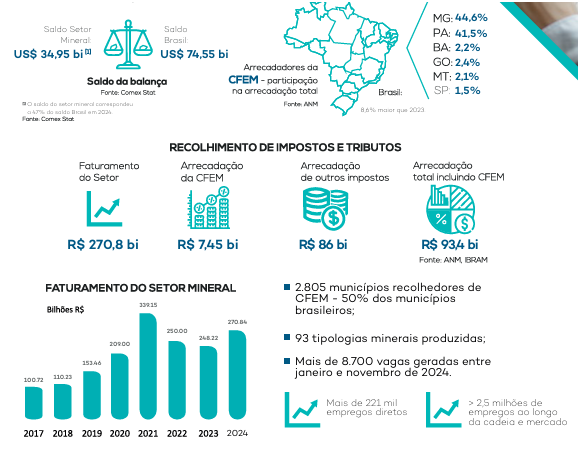
\includegraphics[width=\textwidth]{figures/mineracao_numeros_1.png}
    \caption{Mineração em Números (2024) -- Saldo comercial, impostos e faturamento}
    \label{fig:mineracao_numeros_1}
    \fonte{Mineração em Números (IBRAM, 2024)}
\end{figure}

\begin{figure}[htb]
    \centering
    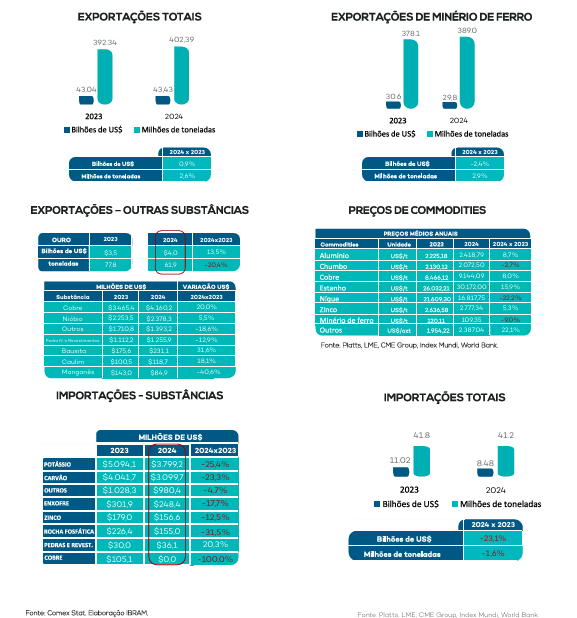
\includegraphics[width=\textwidth]{figures/mineracao_numeros_2.png}
    \caption{Mineração em Números (2024) -- Exportação e Importação}
    \label{fig:mineracao_numeros_2}
    \fonte{Mineração em Números (IBRAM, 2024)}
\end{figure}

\begin{figure}[htb]
    \centering
    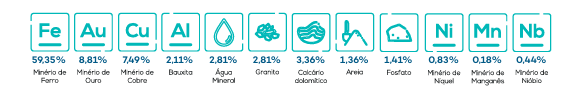
\includegraphics[width=\textwidth]{figures/mineracao_numeros_3.png}
    \caption{Mineração em Números (2024) -- Principais substâncias produzidas -- Participação no faturamento do setor}
    \label{fig:mineracao_numeros_3}
    \fonte{Mineração em Números (IBRAM, 2024)}
\end{figure}

\subsubsection{Geração de empregos}
\label{subsubsec:geracao_empregos}

